\documentclass[11pt,usenames]{article}
\usepackage{srcltx,pdfsync}
%\usepackage[pdflatex=false,recompilepics]{gastex} 
\usepackage{amsmath,amssymb,amsfonts}
\usepackage{color}
\usepackage{hyperref, url}
\usepackage{geometry}
\usepackage{graphicx,subfigure,wrapfig}
\geometry{verbose,a4paper,tmargin=30mm,bmargin=50 mm,lmargin=25mm,rmargin=16mm}
\usepackage{ifthen}

\def\Lap{\ensuremath{\mathcal{L}}}
\usepackage{fancyhdr}
\pdfpagewidth 8.5in
\pdfpageheight 11in

\pagestyle{fancy}
\headheight 35pt


\graphicspath{{../7_Images/}}

%%%%%%%%%%%%%
\usepackage[fancythm]{jphmacros2e}
\renewcommand{\footrulewidth}{0.5 pt}

\rhead{\small{Project Report}}
\chead{}
\lhead{\small{EML 5311}}
\lfoot{Ninad Gaikwad}
\cfoot{\thepage}
\rfoot{}

\title{}

\date{}
\begin{document}

\begin{center}
{\sc Control Systems Theory}\\
University of Florida \\
 Mechanical and Aerospace Engineering
\vspace{0.5 cm}
\end{center}

{\large \begin{center}
	\textbf{Project - Report}\\
	Design and testing of State Feedback based Set-Point Tracking Controller
\end{center}}


\section{System Identification}
The Sine sweep method is used for system identification. In this method the real plant is fed with a bunch of sinusoidal inputs at frequencies which sweep the entire frequency spectrum of the plant operation. The output of the real plant for each of the sinusoidal input is used to create the frequency response of the real plant. From this frequency response we estimate the plant transfer function which is then used for controller design.\\
However, the real plant can be in any initial state other than zero when the sine sweep experiment is started; and hence the plant output will take some finite time to settle to a steady-state. It is this steady-state value of the output for a given sinusoidal input which is required for frequency response computation. Also, even after the output of the plant has reached steady-state there is noise in the measured output due to sensor noise which can lead to incorrect computation of the frequency response.
Therefore, we need to tackle the problem of unknown initial states and sensor noise for getting a good frequency response of the real plant from the sine sweep experiment.

\subsection{ Overcoming Effect of Initial States and Sensor Noise}

\begin{enumerate}
	
	\item \textbf{Effect of Initial States:} To mitigate the effect initial states on the output of the plant, we need to keep an initial buffer time so that the plant reaches steady state. This decay time can be found out by running the plant in open-loop using a bunch of sinusoidal inputs representative of the entire spectrum and measuring the time when the output reaches steady state. Fig.\ref(fig:EffectOfInitialStates) illustrates the open-loop response of the plant, it can be seen that for the given range of frequencies (1 rad/s, 10 rad/s, 100 rad/s and 500 rad/s) the \textbf{Decay Time = 30 sec}.
	
	\begin{figure}[htpb]
		\centering
		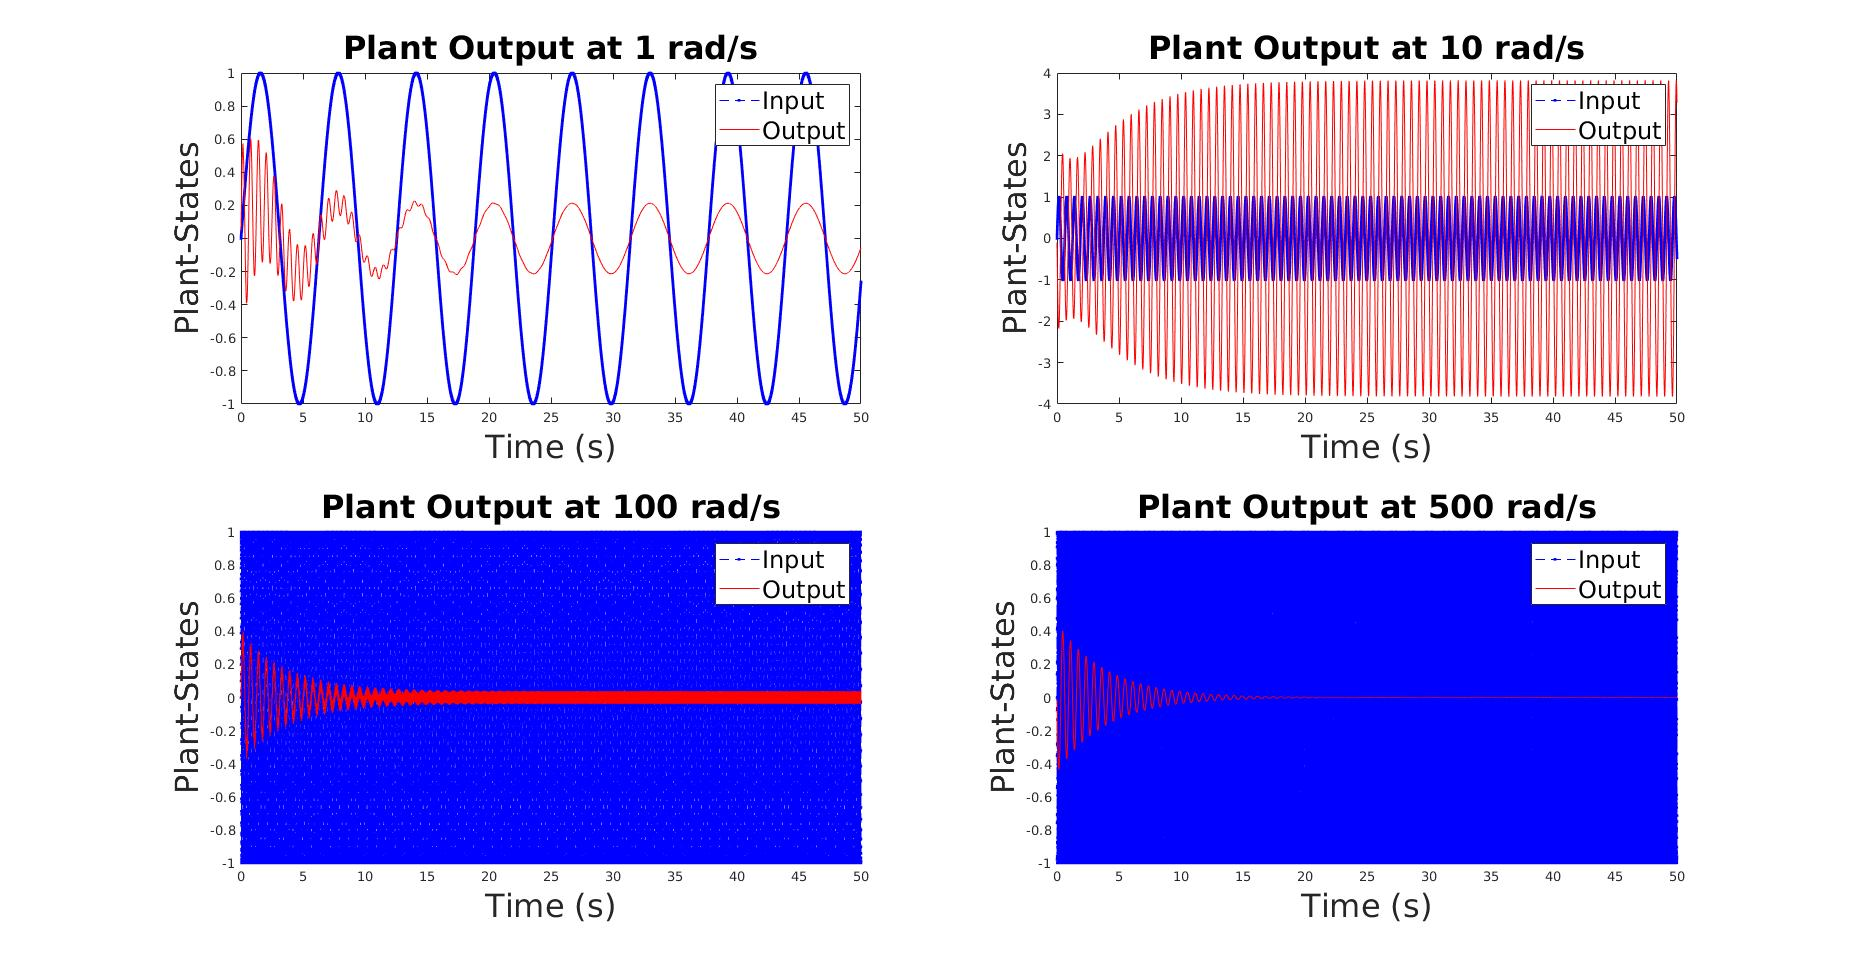
\includegraphics[width=1\columnwidth]{EffectOfInitialStates.jpg}
		\caption{Plant reaches Steady-State before 30 seconds for the entire spectrum of frequencies}
		\label{fig:EffectOfInitialStates}
	\end{figure}	
	
	\item \textbf{Effect Sensor Noise:} To mitigate the effect of sensor noise on the corruption of steady state output measurement of the plant; the number of cycles of the measured output which are used in the sine sweep algorithm are kept large. This is because the sensor noise is a zero mean signal; and if we measure enough data points of a noisy signal corrupted by a zero mean signal, then the mean of this signal is independent of the noise and truly represents the mean of the real signal. Hence, using large number of cycles of the plant output at steady state helps us in computing the frequency response accurately. For the results in this report the  \textbf{Cycles = 25}.
	
\end{enumerate}

\subsection{Frequency Response and Transfer Function Estimation}

The following parameters were selected for running the sine sweep experiment on the plant;

\begin{enumerate}
	\item Input Frequencies: 30 frequencies ranging between 0.1 - 500 
	\item Decay Time: 30 seconds
	\item Number of Cycles to Average: 25
	\item Sampling Frequency: 1000 Hz (selected to be twice of the maximum input sinusoid frequency [Nyquist Sampling Criteria] )
\end{enumerate}

The Fig.\ref{fig:NominalSineSweep} shows the nominal frequency response of the plant obtained from the sine sweep experiment. It can be seen that there is a pair of complex conjugate zeros at $ \omega_z = 30 rad/s $ and two pairs of complex conjugate poles at $ \omega_{p1} = 10 rad/s $ and $ \omega_{p2} = 80 rad/s $ respectively. The unsual $ 360^{\circ} $ jump after $ 100 rad/s $ is not substantiated by $ +80db/dec $ as we would expect if there were actual two pairs of complex conjugate zeros hence that phase shift can be ignored.
  
\begin{figure}[htpb]
	\centering
	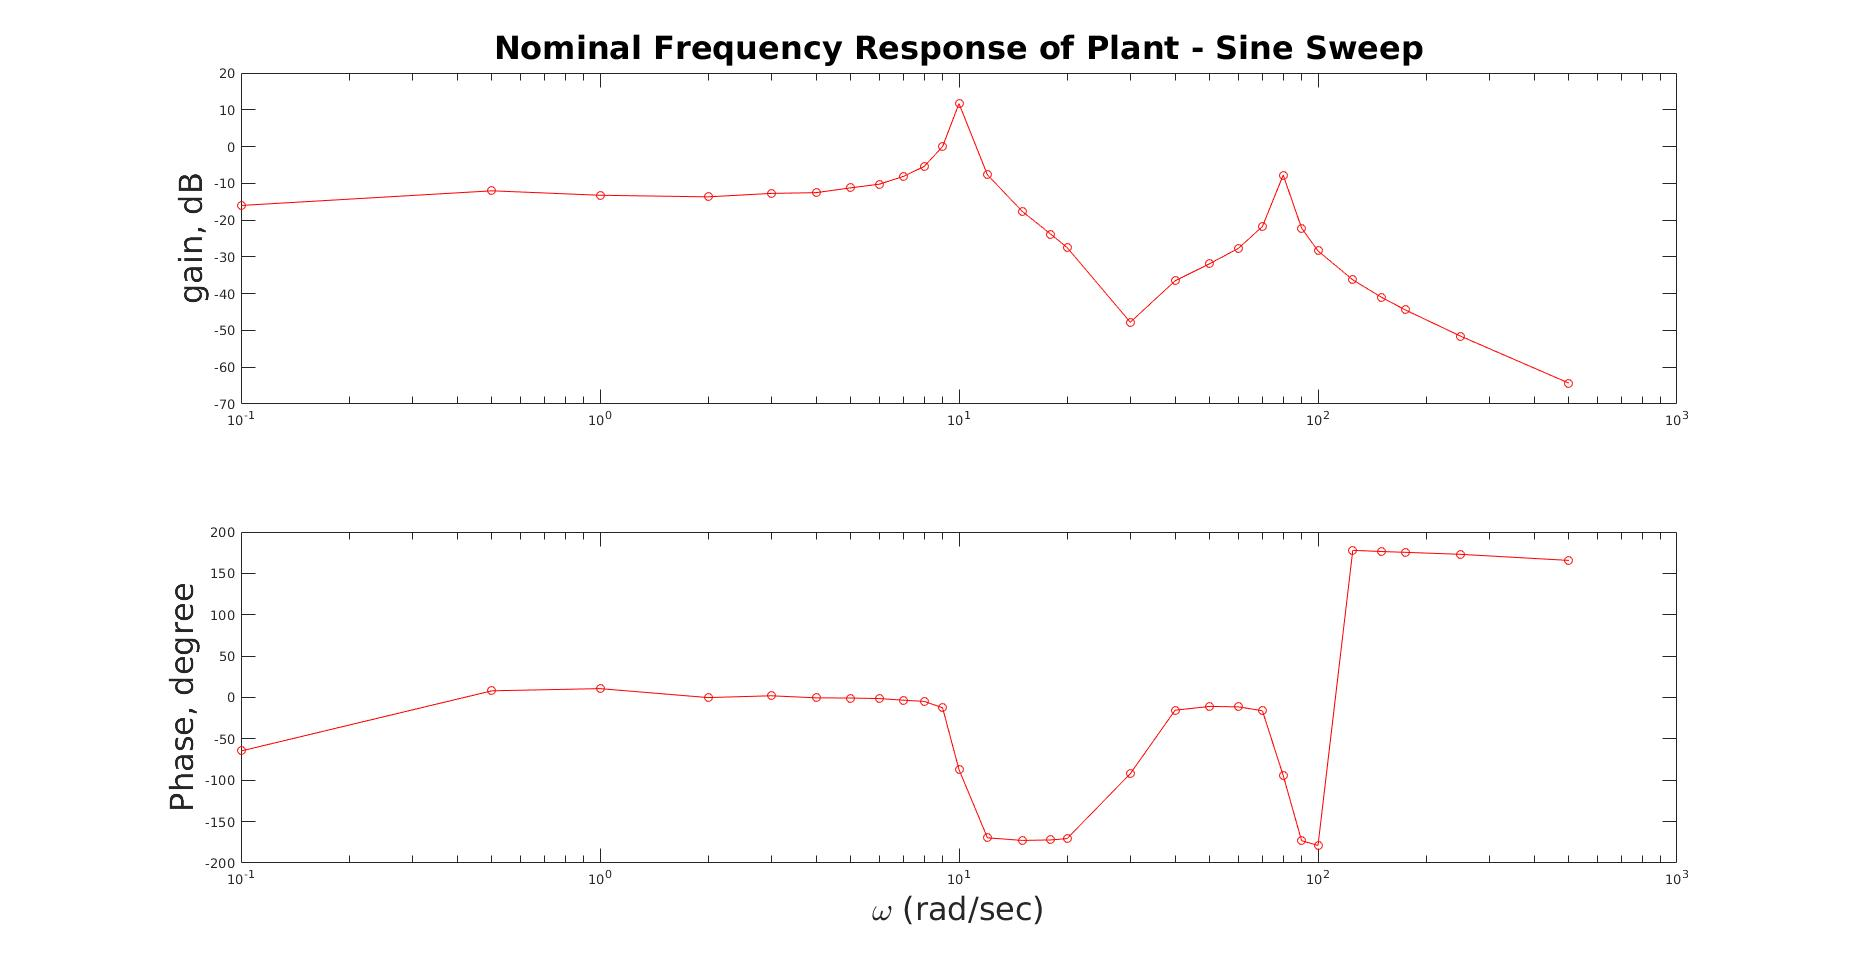
\includegraphics[width=1\columnwidth]{NominalSineSweep.jpg}
	\caption{Nominal Frequency Response of the Plant}
	\label{fig:NominalSineSweep}
\end{figure}

Two methods for estimating the transfer function were used, the first one includes using the in built MATLAB function invfreqs() which takes in the complex frequency response of the plant computed in the sine sweep and the transfer function numerator and denominator values to give out the best fit transfer function model. 
The transfer function computed from this method is as follows;

\begin{equation} 
\hat{P_{\circ}}(s)=\dfrac{143.2s^{2}+12860s+91230}{s^{4}+5.742s^{3}+6870s^{2}+905.2s+644200}
\label{eq:Ginv}
\end{equation}

However, as can be seen from the Fig.\ref{fig:SineSweepVsEstimatedTFs} it is not able to satisfactorily estimate the behavior of the pair of complex conjugate zeros. Hence, a heuristic method was used to determine the best fit Transfer Function for the plant.

\subsubsection{Heuristic Method for Estimating Best Fit Transfer Function}
As it is evident from Fig.\ref{fig:NominalSineSweep} that there is a pair of complex conjugate zeros at $\omega_z = 30 rad/s$ and two pairs of complex conjugate poles at $\omega_{p1} = 10 rad/s$ and $\omega_{p2} = 80 rad/s$ respectively, the transfer function model can be modeled as follows;

\begin{equation} 
\hat{P_{\circ}}(s)=\dfrac{k_{1}(s^{2}+2\zeta_{1}\omega_{z1}s+\omega_{z1}^{2})}{(s^{2}+2\zeta_{2}\omega_{p1}s+\omega_{p1}^{2})k_{1}(s^{2}+2\zeta_{3}\omega_{p2}s+\omega_{p2}^{2})}
\label{eq:TF1}
\end{equation}

where; $ zeta_{1}, zeta_{2}, zeta_{3}$ are the damping ratios. Now, $k_{1}$ can be determined from  and $\lvert G(j\omega) \rvert _{\omega=0}$ available from the sine sweep experiment and \eqref{eq:TF1} by putting $ s=j\omega=0 $. However, as the sine sweep was taking too long to compute values at $ \omega=0 $ this approximation was used, $ \lvert G(j\omega) \rvert _{\omega=0} \approx \lvert G(j\omega) \rvert _{\omega=0.1}$. However, this resulted in a constant bias between the  

\begin{equation} 
k_{1}=\dfrac{\lvert \hat{P_{\circ}}(j\omega) \rvert _{\omega=0} \omega_{p1}^{2} \omega_{p2}^{2} }{\omega_{z1}^{2}}
\label{eq:TF2}
\end{equation}

$k_{1}=150.4966$ is computed from the above procedure. Now we have to find best combination of   $ (\zeta_{1}, \zeta_{2}, \zeta_{3}) $ and this was done heuristically in the following manner;

\begin{enumerate}
	\item Create combinations of $ (\zeta_{1}, \zeta_{2}, \zeta_{3}) $ spanning the entire range  $ 0 \leq \zeta \leq 1 $ with computationally feasible discretization.
	\item For a given combination of $ (\zeta_{1}, \zeta_{2}, \zeta_{3}) $ and already computed $k_{1}$ value the transfer function given in \eqref{eq:TF1} is created.
	\item Frequency response of this transfer function is computed at frequencies for which sine sweep experiment was conducted.
	\item Root mean squared error (RMSE) is computed for the magnitude response
	\item Steps 2 to 4 are repeated for all the combinations of $ (\zeta_{1}, \zeta_{2}, \zeta_{3}) $.
	\item The transfer function model with the least magnitude response RMSE is chosen as the best fit model.
\end{enumerate}

The Fig.\ref{fig:OpenLoopk1Bias} shows the open loop response of the actual plant against transfer functions estimated using invfreqs() and the heuristic method, it can be clearly seen that the transfer function obtained from the heuristic method is more resembling to the plant output. 

\begin{figure}[htpb]
	\centering
	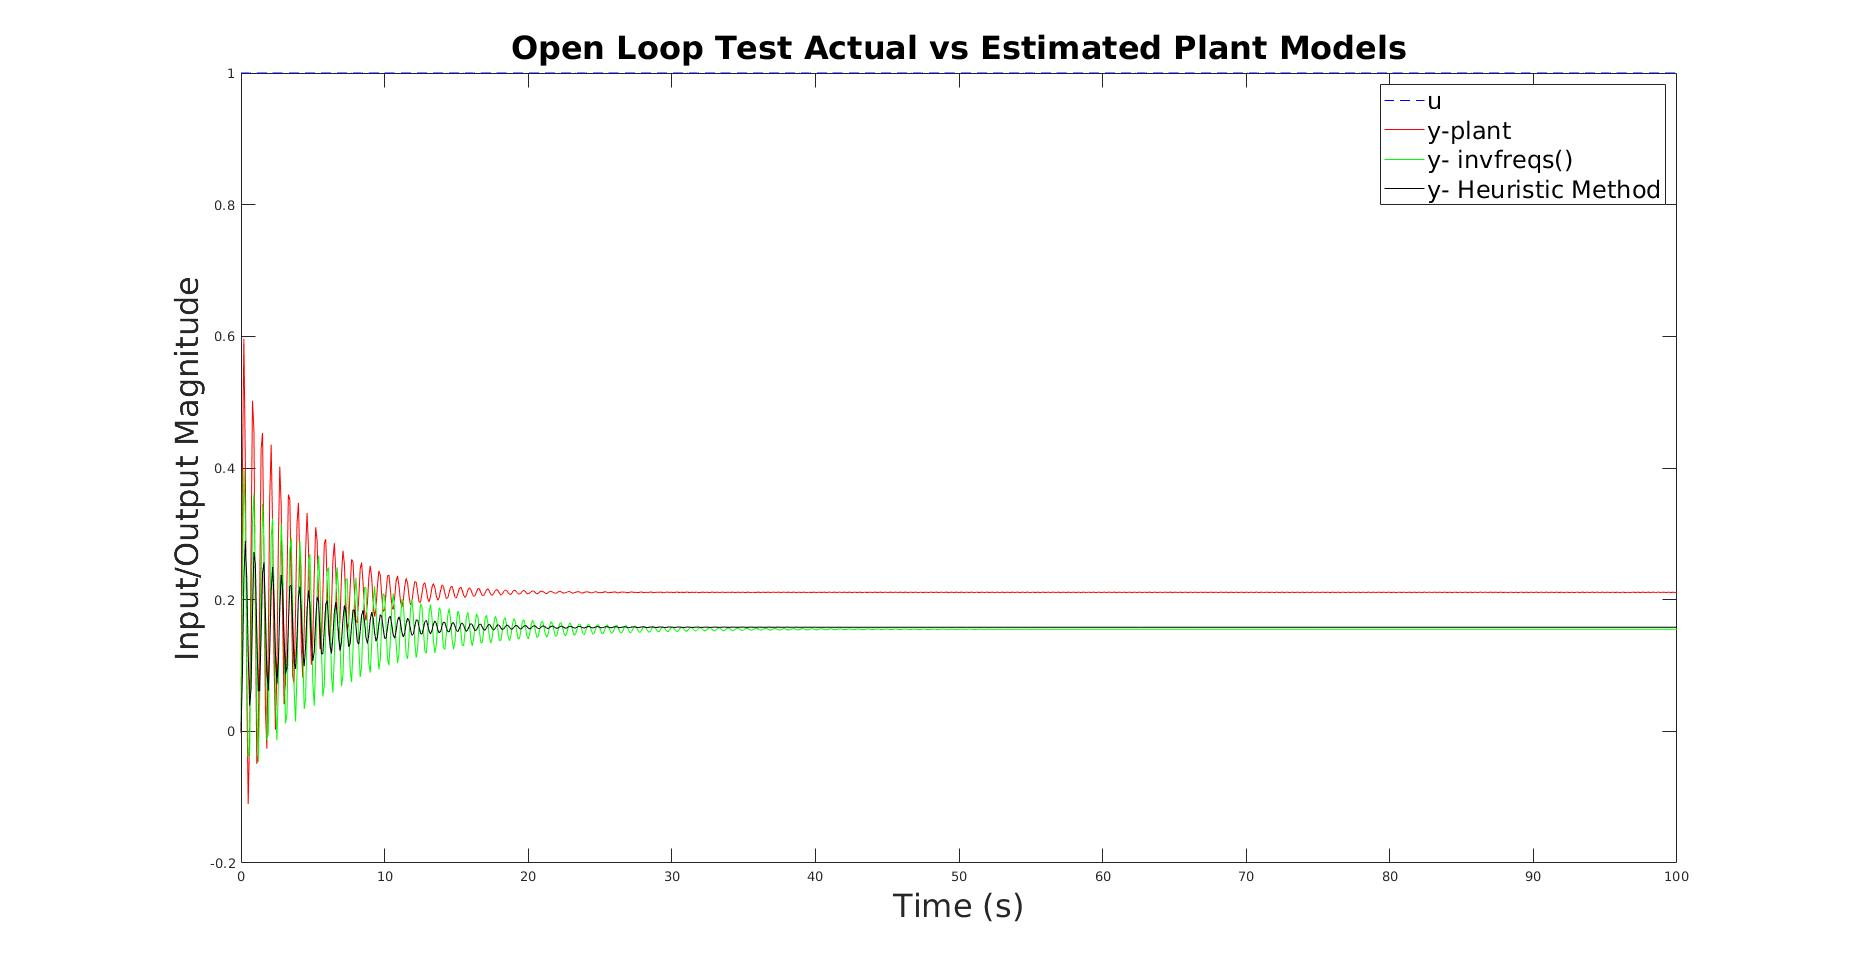
\includegraphics[width=1\columnwidth]{OpenLoopk1Bias.jpg}
	\caption{Open loop test of actual and estimated plants }
	\label{fig:OpenLoopk1Bias}
\end{figure}

Hence, the transfer function estimated from the sine sweep experiment using the heuristic approach is given by \eqref{eq:Gheu} , where the damping ratios are $ (\zeta_{1}=0.1, \zeta_{2}=0.03, \zeta_{3}=0.03) $

\begin{equation} 
\hat{P_{\circ}}(s)=\dfrac{150.5s^{2}+903s+135400}{s^{4}+5.4s^{3}+6503s^{2}+4320s+640000}
\label{eq:Gheu}
\end{equation}

The Fig.\ref{fig:SineSweepVsEstimatedTFs} shows the bode plots of transfer functions estimated from the above mentioned two methods against the sine sweep of the plant. It can be clearly seen that the transfer function estimated using the heuristic method fits the sine sweep better.

\begin{figure}[htpb]
	\centering
	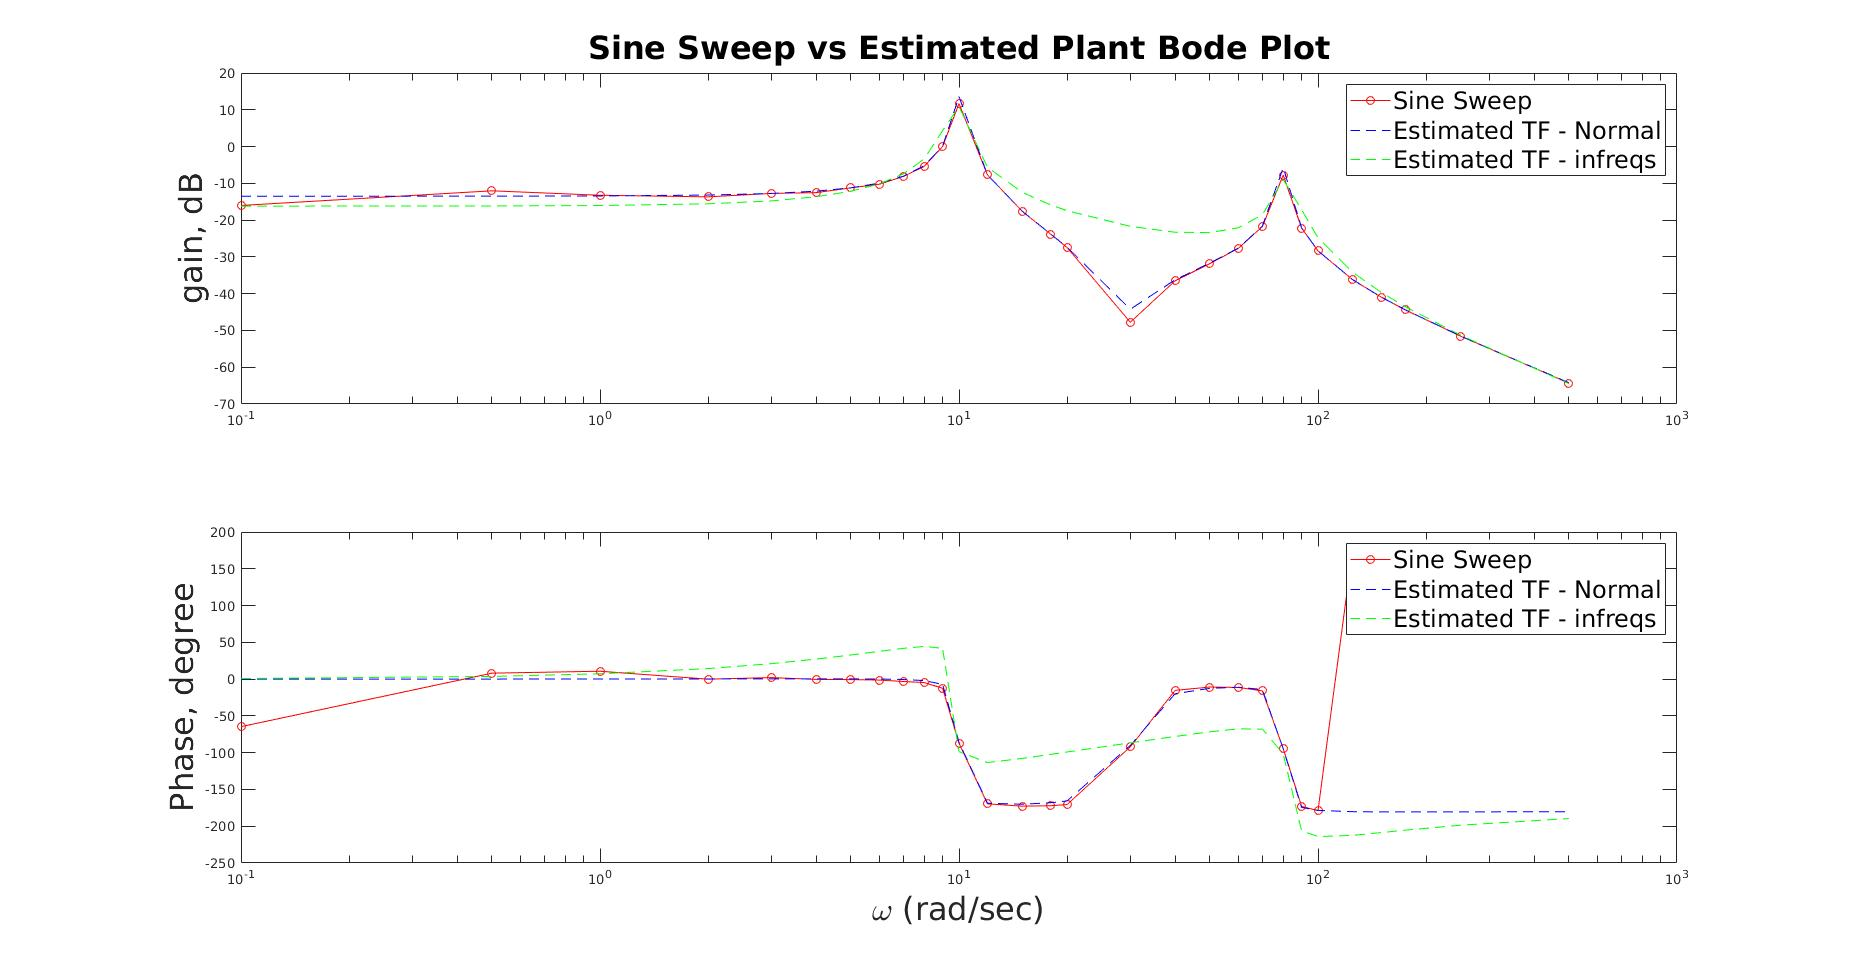
\includegraphics[width=1\columnwidth]{SineSweepVsEstimatedTFs.jpg}
	\caption{ Bode Plot of plant (sine sweep), TF with approximate $k_{1}$ and TF with accurate $k_{1}$ }
	\label{fig:SineSweepVsEstimatedTFs}
\end{figure}

The above transfer function is converted to a state space model in MATLAB with the following $ A, B, C \text{ and } D$ matrices so that state space control techniques can be applied. As state-space model is created from a transfer function, it is a minimal realization.
$$
A = 
\begin{bmatrix} 
	-5.4 & -6502.9 & -4320 & -6.4e+5\\
	0 & 0 & 0 & 0\\
	0 & 0 & 0 & 0\\
	0 & 0 & 0 & 0\\
\end{bmatrix}
,B = 
\begin{bmatrix} 
1 \\
0 \\
0 \\
0 \\ 
\end{bmatrix}
,C = 
\begin{bmatrix} 
0 & 200 & 1210 & 1.8082e+05
\end{bmatrix}
\text{and } D = 
\begin{bmatrix} 
0
\end{bmatrix}
$$

\section{Controller Design}
The control problem: Tracking the given reference signal with performance criteria: peak overshoot of less than $15\%$ and rise time of less than 2 seconds. The controller has to be designed using state-space design techniques. It is evident that this is a set-point tracking problem and the controller will consist of a feedback gain $K$, Luenberger Observer with gain $L$ and the steady-state control command $U^{*}$.

\subsection{Set Point Tracking using Feedback Regulation}
The Fig.\ref{fig:SSController} illustrates the schematic of set-point tracking controller.
 
\begin{figure}[htpb]
	\centering
	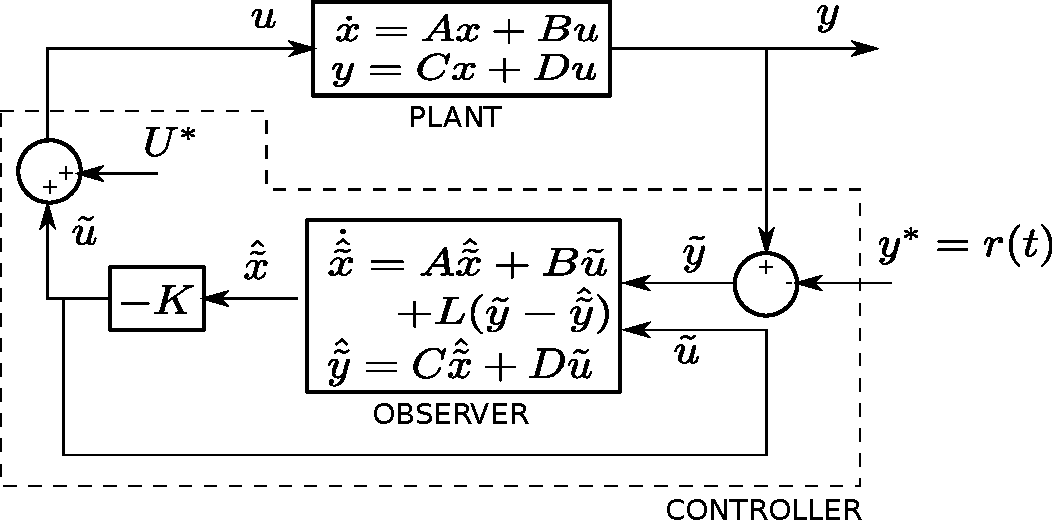
\includegraphics[width=0.65\columnwidth]{SSController_Structure_Image.pdf}
	\caption{ Set Point Tracking using Feedback Regulation - Controller Schematic }
	\label{fig:SSController}
\end{figure}

The plant dynamics are given as follows;

\begin{align}
\dot{x}&=Ax+Bu \\
y&=Cx+Du
\end{align}

We have to perform set-point tracking on the above plant, but we know how to compute feedback gain $K$ and Luenberger Observer gain $L$ for performing state regulation on the above plant dynamics. From the given data we know the steady-state equations for the above plant will be as follows, where $X^{*}$ and $U^{*}$ are the steady-state values of the states and the control commal respectively;

\begin{align}
AX^{*}+BU^{*}&=0 \\
CX^{*}+DU^{*}&=r_{\circ}\\\hat{P_{\circ}}(s)
\begin{bmatrix}
A & B\\
C & D
\end{bmatrix} 
\begin{bmatrix}
X^{*} \\
U^{*} 
\end{bmatrix} &= 
\begin{bmatrix}
0 \\
r_{\circ}
\end{bmatrix}\\
\begin{bmatrix}
X^{*} \\
U^{*} 
\end{bmatrix} &=
\begin{bmatrix}
A & B\\
C & D
\end{bmatrix}^{-1} 
\begin{bmatrix}
0 \\
r_{\circ}
\end{bmatrix}
\end{align}

Hence we would define the following new states (co-ordinate transformation) for converting the set-point tracking problem to a state regulation problem;

\begin{align}
\tilde{x}&=x-X^{*} \\
\tilde{y}&=y-r_{\circ} \\
\tilde{u}&=u-U^{*} 
\end{align} 

Knowing that $X^{*}$, $U^{*}$ and $r_{\circ}$ are constants their derivatives are zeros, and then using equations (13),(14),(15),(10) and (9) in the plant dynamic equations (7) and (8), we derive the transformed plant dynamics as follows; and they are exactly equal to the actual plant dynamics.

\begin{align}
\dot{\tilde{x}}&=A\tilde{x}+B\tilde{u} \\
\tilde{y}&=C\tilde{x}+D\tilde{u}
\end{align}

Now we can design feedback gain $K$ ($A,B$ have to be completely controllable)  using LQR (Linear Quadratic Regulator - helps in computing gain $K$ which can both bring the states to zero in some finite time while keeping the control command within bounds, lqr()-MATLAB function) and then come up with a Luenberger Observer gain $L$ ($A,C$ have to be completely observable) with the place()-MATLAB function such that the observer poles (eigenvalues of $A-LC$) are 5-10 times that of the controller poles (eigenvalues of $A-BK$) and  hence perform state regulation on the transformed plant dynamics as illustrated in Fig.\ref{}. We can easily see that at steady-state under the effect of the state feedback controller $\tilde{x} \rightarrow 0$, $\tilde{y} \rightarrow 0$ and $\tilde{u} \rightarrow 0$ which correspond to $x \rightarrow X^{*}$, $y \rightarrow r_{\circ}$ and $u \rightarrow U^{*}$

\begin{figure}[htpb]
	\centering
	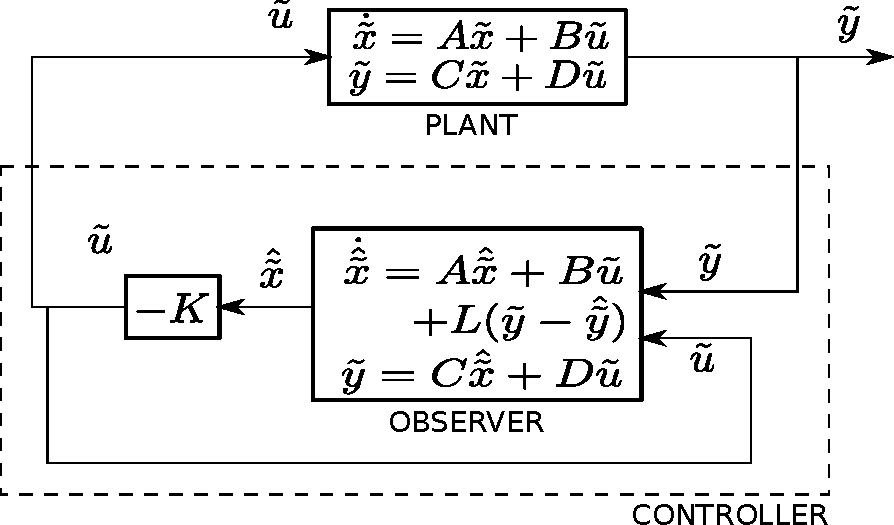
\includegraphics[width=0.60\columnwidth]{LQRControllerFBStateRegulation_Image.pdf}
	\caption{ Feedback State Regulation on transformed Plant - Schematic }
	\label{fig:LQRControllerFBStateRegulation_Image}
\end{figure}

The closed loop system for the state regulation is given as follows; first defining a new state and the input as,

\begin{align} 
e&=\tilde{x}-\hat{\tilde{x}}\\ 
\tilde{u}&=-K\hat{\tilde{x}}
\end{align}

Now using equations (18), (19) in (16), (17) (Transformed Plant Dynamics) and (7), (8) (Actual Plant Dynamics), we get;

\begin{align} 
\dot{x}&=(A-BK)x+BKe\\
\dot{e}&=(A-LC)\\
\begin{bmatrix}
\dot{x}\\
\dot{e}
\end{bmatrix} &=
\begin{bmatrix}
A-BK & BK \\
0 & A-LC
\end{bmatrix}
\begin{bmatrix}
x\\
e
\end{bmatrix} 
\end{align}

As the closed loop dynamics of the state regulation are block diagonal in structure, hence gain $K$ and $L$ can be independently designed (separation principle) as long as ($A,B$) and ($A,C$) are completely controllable and observable respectively. From equation (22) it can be seen that $\tilde{x} \rightarrow 0$, $e \rightarrow 0$ if eigenvalues of $(A-BK)$ and $(A-LC)$ are in the SLHP (Strict Left Half-Plane).

\subsection{Loop Transfer Function of the State Space Design}

The Fig.ref{fig:SSController} is slightly modified to give Fig.(fig:SSOpenLoop) , here we can see the state space systems connected as $C(s)$ = Controller and $P(s)$ = Plant. We can find out the transfer function from the state space models with the shown input - output characteristics.

\begin{figure}[htpb]
	\centering
	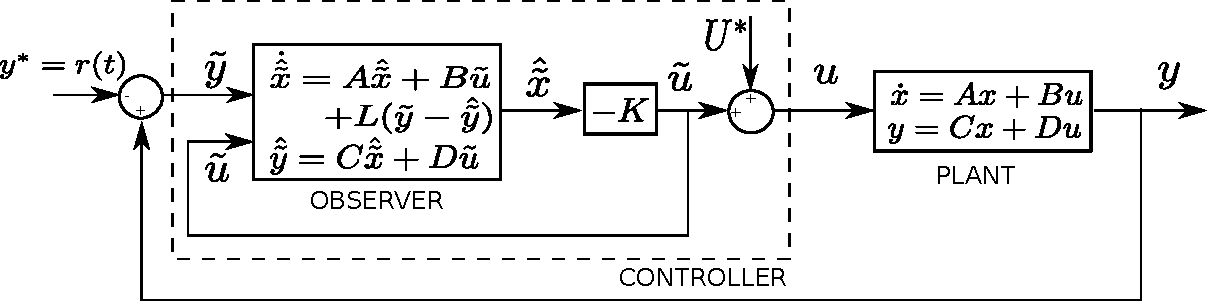
\includegraphics[width=0.75\columnwidth]{SSController_OpenLoopTF_Image.pdf}
	\caption{ Set Point Tracking using Feedback Regulation - Modified Controller Schematic }
	\label{fig:SSOpenLoop}
\end{figure}

The transfer function of the plant between input signal $u(s)$ and output signal $y(s)$ is given by from equations;

\begin{align} 
P(s)&=Cdet(sI-A)^{-1}B
\end{align}

Whereas, the transfer function of the controller between input signal $\tilde{y}(s)$ and output signal $\tilde{u}(s)$ and omitting the feed-forward term in its output equation as well as omitting $U^{*}$ is given by;

\begin{align}
&\text{Observer Dynamics:}\\
\dot{\hat{\tilde{x}}}&=(A-BK-LC)\hat{\tilde{x}}+L\tilde{y} \\
\tilde{u}&=-K\hat{\tilde{x}} \\
&\text{Hence,}\\
C(s)&=Kdet(sI-A+BK+LC)^{-1}L
\end{align}

Therefore the loppf transfer function $L(s)=C(s)P(s)$ is given by;

\begin{align} 
L(s)&=\left[ Kdet(sI-A+BK+LC)^{-1}L\right] \left[ Cdet(sI-A)^{-1}B\right] 
\end{align}

The stability margins obtained from the margin() - MATLAB function for $L(s)$ are;

\begin{enumerate}
	\item $GM = 17.61$
	\item $PM = 91.88^{\circ}$
	\item $W_{cg} = 220.23^{\circ}$
	\item $W_{cp} = 89.35^{\circ}$
\end{enumerate}

Hence, the closed loop system is stable and has a good buffer of $GM$ (Gain Margin) and $PM$ (Phase Margin), which tells us that the system is robust to modeling errors and will not drive into instability till the margins are violated.

\subsection{Design Testing}
The controller based on state-space design techniques is first designed and tested for the estimated plant transfer function ($\hat{P_{\circ}}(s)$), the method followed is as follows;

\begin{enumerate}
	\item Convert the estimated transfer function eq(6) to its equivalent state-space model.
	\item Choose appropriate $Q$ and $R$ matrices (in our case scalars) such that design specifications are met. Higher the value of $Q$ more the state magnitudes are penalized and hence they settle more quickly, but this can increase the control effort and the control command can get saturated. Higher the value of $R$ more is the control command penalized and it will not get saturated, but this will reduce control effort causing the output to settle after a long time. Hence an optimal trade-off between the  $Q$ and $R$ values have to be reached to extract optimal performance.
	\item Apply LQR for computing appropriate $K$ matrix for feedback regulation (lqr()-MATLAB function).
	\item Compute the controller poles i.e. the poles of $A-BK$.
	\item Compute the observer poles i.e. poles of $A-LC$ as 5-10 times that of controller poles (in our only real part of the controller poles are used, as large imaginary parts can lead to poor observer performance)
	\item Now use the pole-placement method to compute the appropriate $L$ for the observer (place() - MATLAB function).
	\item Run the design simulation for the given reference signal and observe the performance.
	\item Repeat steps 2 through 7 till desired closed loop performance is achieved.	
\end{enumerate}

\begin{figure}[htpb]
	\centering
	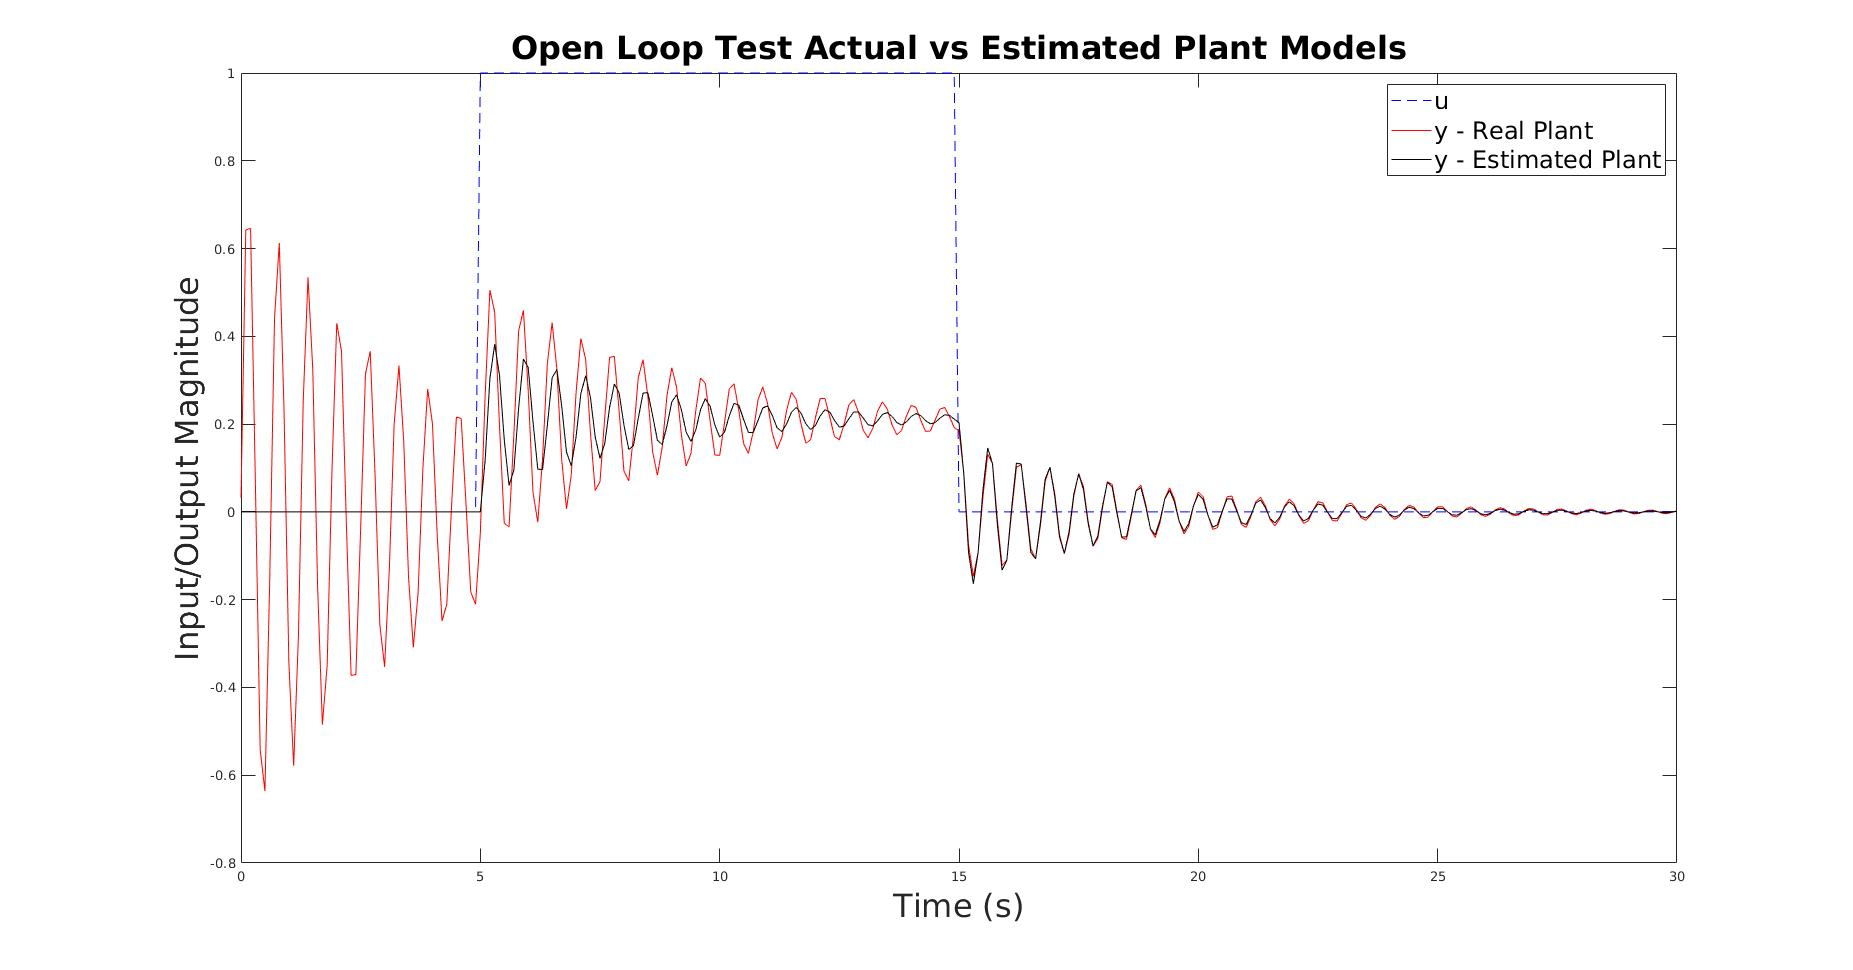
\includegraphics[width=0.85\columnwidth]{OpenLoop_PlantTF.jpg}
	\caption{Open Loop behavior of actual and estimated plant for the given reference signal}
	\label{fig:OpenLoop_PlantTF}
\end{figure}

The Fig.\ref{fig:OpenLoop_PlantTF} shows the open loop behavior of the actual plant and estimated model. It can be observed that, both the models have a poor performance in tracking the step reference as the seem to be settling very slowly to a much lower value. This should be improved with our closed loop feedback controller. (Note: the estimated model seems to be tracking the initial zero reference accurately because it starts from zero initial states and the actual plant starts from random initial states)



The Controller design parameters are as follows:

\begin{enumerate}
	\item $D = \left[ 1 \quad1\quad 1\quad 1\right] $
	\item $Q = 400000$
	\item $R = 500$
	\item $K = \left[24.47 \quad31.59 \quad3367.2 \quad6.25e-04\right]$	
	\item $L = \left[201.9326 \quad-0.2904 \quad0.0261 \quad0.0026\right] $
\end{enumerate}

\begin{figure}[htpb]
	\centering
	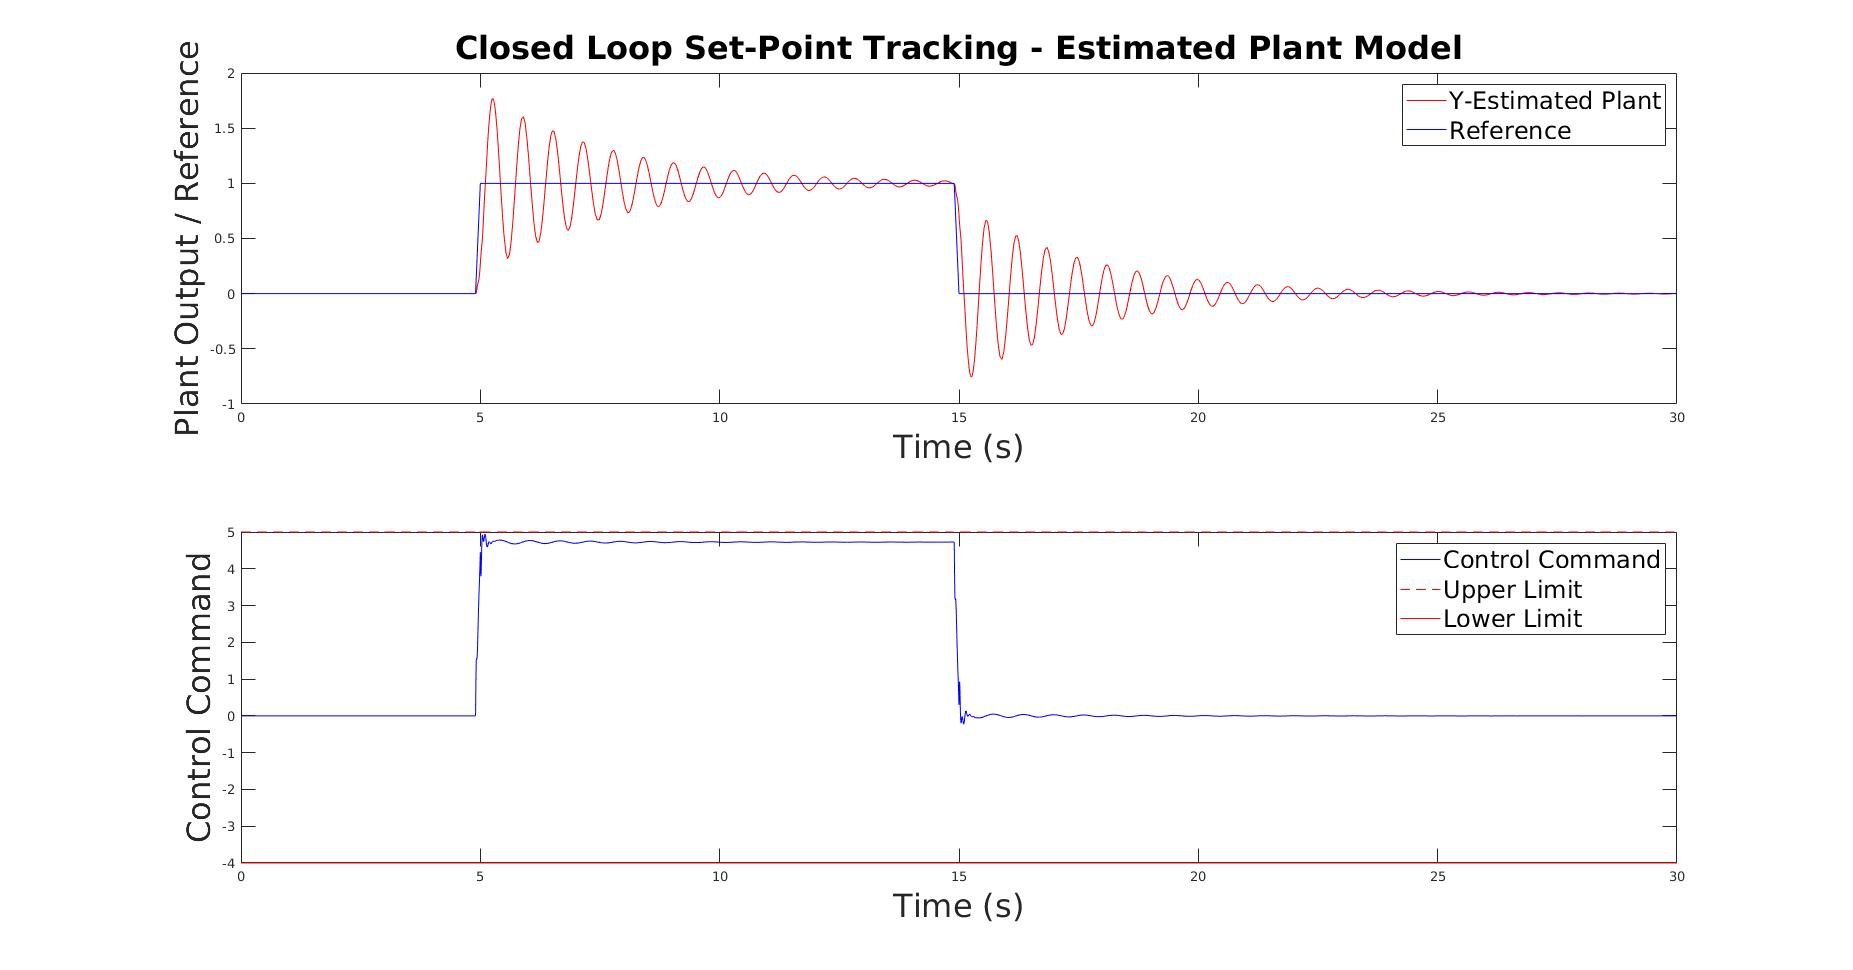
\includegraphics[width=0.85\columnwidth]{ClosedLoop_Design_OutputRef.jpg}
	\caption{Closed loop behavior of the estimated plant with state feedback based set-point tracking}
	\label{fig:ClosedLoop_Design_OutputRef}
\end{figure}

Fig.\ref{fig:ClosedLoop_Production_OutputRef} illustrates the closed loop behavior of the estimated plant model. It can be seen that rise time is less than 2 seconds and the control command does not saturate; however, the max overshoot is more than $15\%$.

\subsection{Production Test}

The same controller parameters were used on the actual plant, and the closed loop behavior is illustrated in Fig.\ref{fig:ClosedLoop_Production_OutputRef}. It can be seen that the response is similar to the closed loop behavior of the estimated plant model. The rise time is less than 2 seconds and the control command does not saturate; however, the max overshoot is more than $15\%$.

\begin{figure}[htpb]
	\centering
	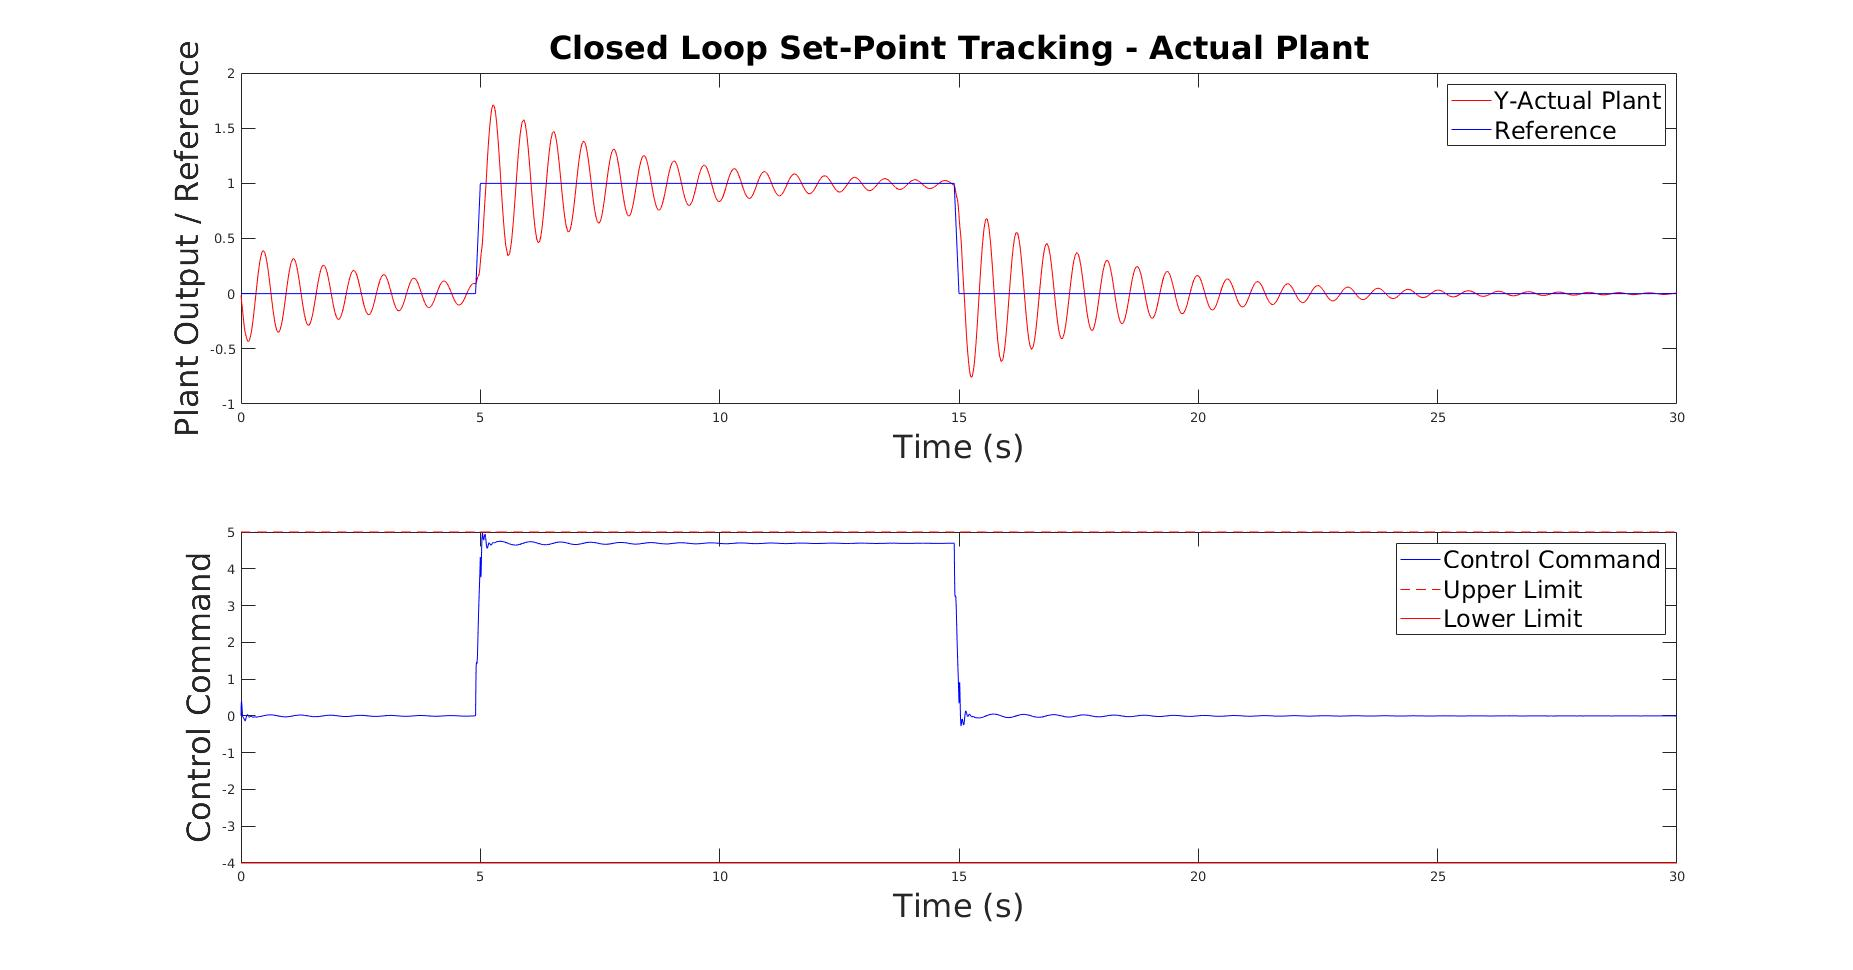
\includegraphics[width=0.85\columnwidth]{ClosedLoop_Production_OutputRef.jpg}
	\caption{Closed loop behavior of the actual plant with state feedback based set-point tracking}
	\label{fig:ClosedLoop_Production_OutputRef}
\end{figure}

\newpage
\section{Conclusion}

Sine sweep experiment was performed to estimate the Transfer Function of an unknown plant. A set-point tracking controller was designed using state-space design techniques. Finally, the closed loop controller performed better than the open loop system response for both the estimated and actual plant. However, only two of three design criterion s were met: Controll command was limited between $+5$ and $-4$ and the rise time was less than 2 seconds. But, the max overshoot for both the plant and estimated model were greater than the desired $15\%$. The reasons for the third criteria not being met, is because of the limits on the control command. If the limits on the control command are removed then it is possible to lower the max overshoot. Otherwise, some other suitable control law has to be used. 

\end{document}










\begin{equation} 
\sum_{k=0}^n k = 1 + 2 + 3 + \cdots + n = \dfrac{n(n+1)}{2}
\label{eq:Pn}
\end{equation}

%% Single Figure Environment
\begin{figure}[htpb]
	\centering
	\includegraphics[width=1\columnwidth]{PCN_BaseStation_SoftwareWorkFlow_Basic.pdf}
	\caption{Flywheel Control System}
	\label{fig:FlywheelCSReal}
\end{figure}

%% Group of Equations
\begin{align*}
\sum_{k=0}^{n+1} k &= \left(\sum_{k=0}^{n} k\right) + (n+1) &\mbox{(sum definition)}\\
&= \frac{n(n+1)}{2} + (n+1) &\mbox{(induction hypothesis)}
\\
&= \frac{n(n+1)}{2} + \frac{2n+2}{2} &\mbox{(common denominator)}
\\
&= \frac{n^2 +n}{2} + \frac{2n+2}{2} &\mbox{(distribute)}
\\
&= \frac{n^2 +3n + 2}{2} &\mbox{(combine like terms)}
\\
&= \frac{(n+1)(n+2)}{2} & \mbox{(factor the numerator)}\\
\end{align*}

In all Fig.\ref{fig:FlywheelCSReal} cases, \eqref{eq:Pn} is true, so $\forall n\in \N$, 
$\Disp \sum_{k=0}^n k = \dfrac{n(n+1)}{2}$